
%\graficarPDFa{02cm 02cm 02cm 02cm}{graf_ej2}{Estimación de la trayectoria.}{fig:ej2}
\begin{figure}[H]
\centering
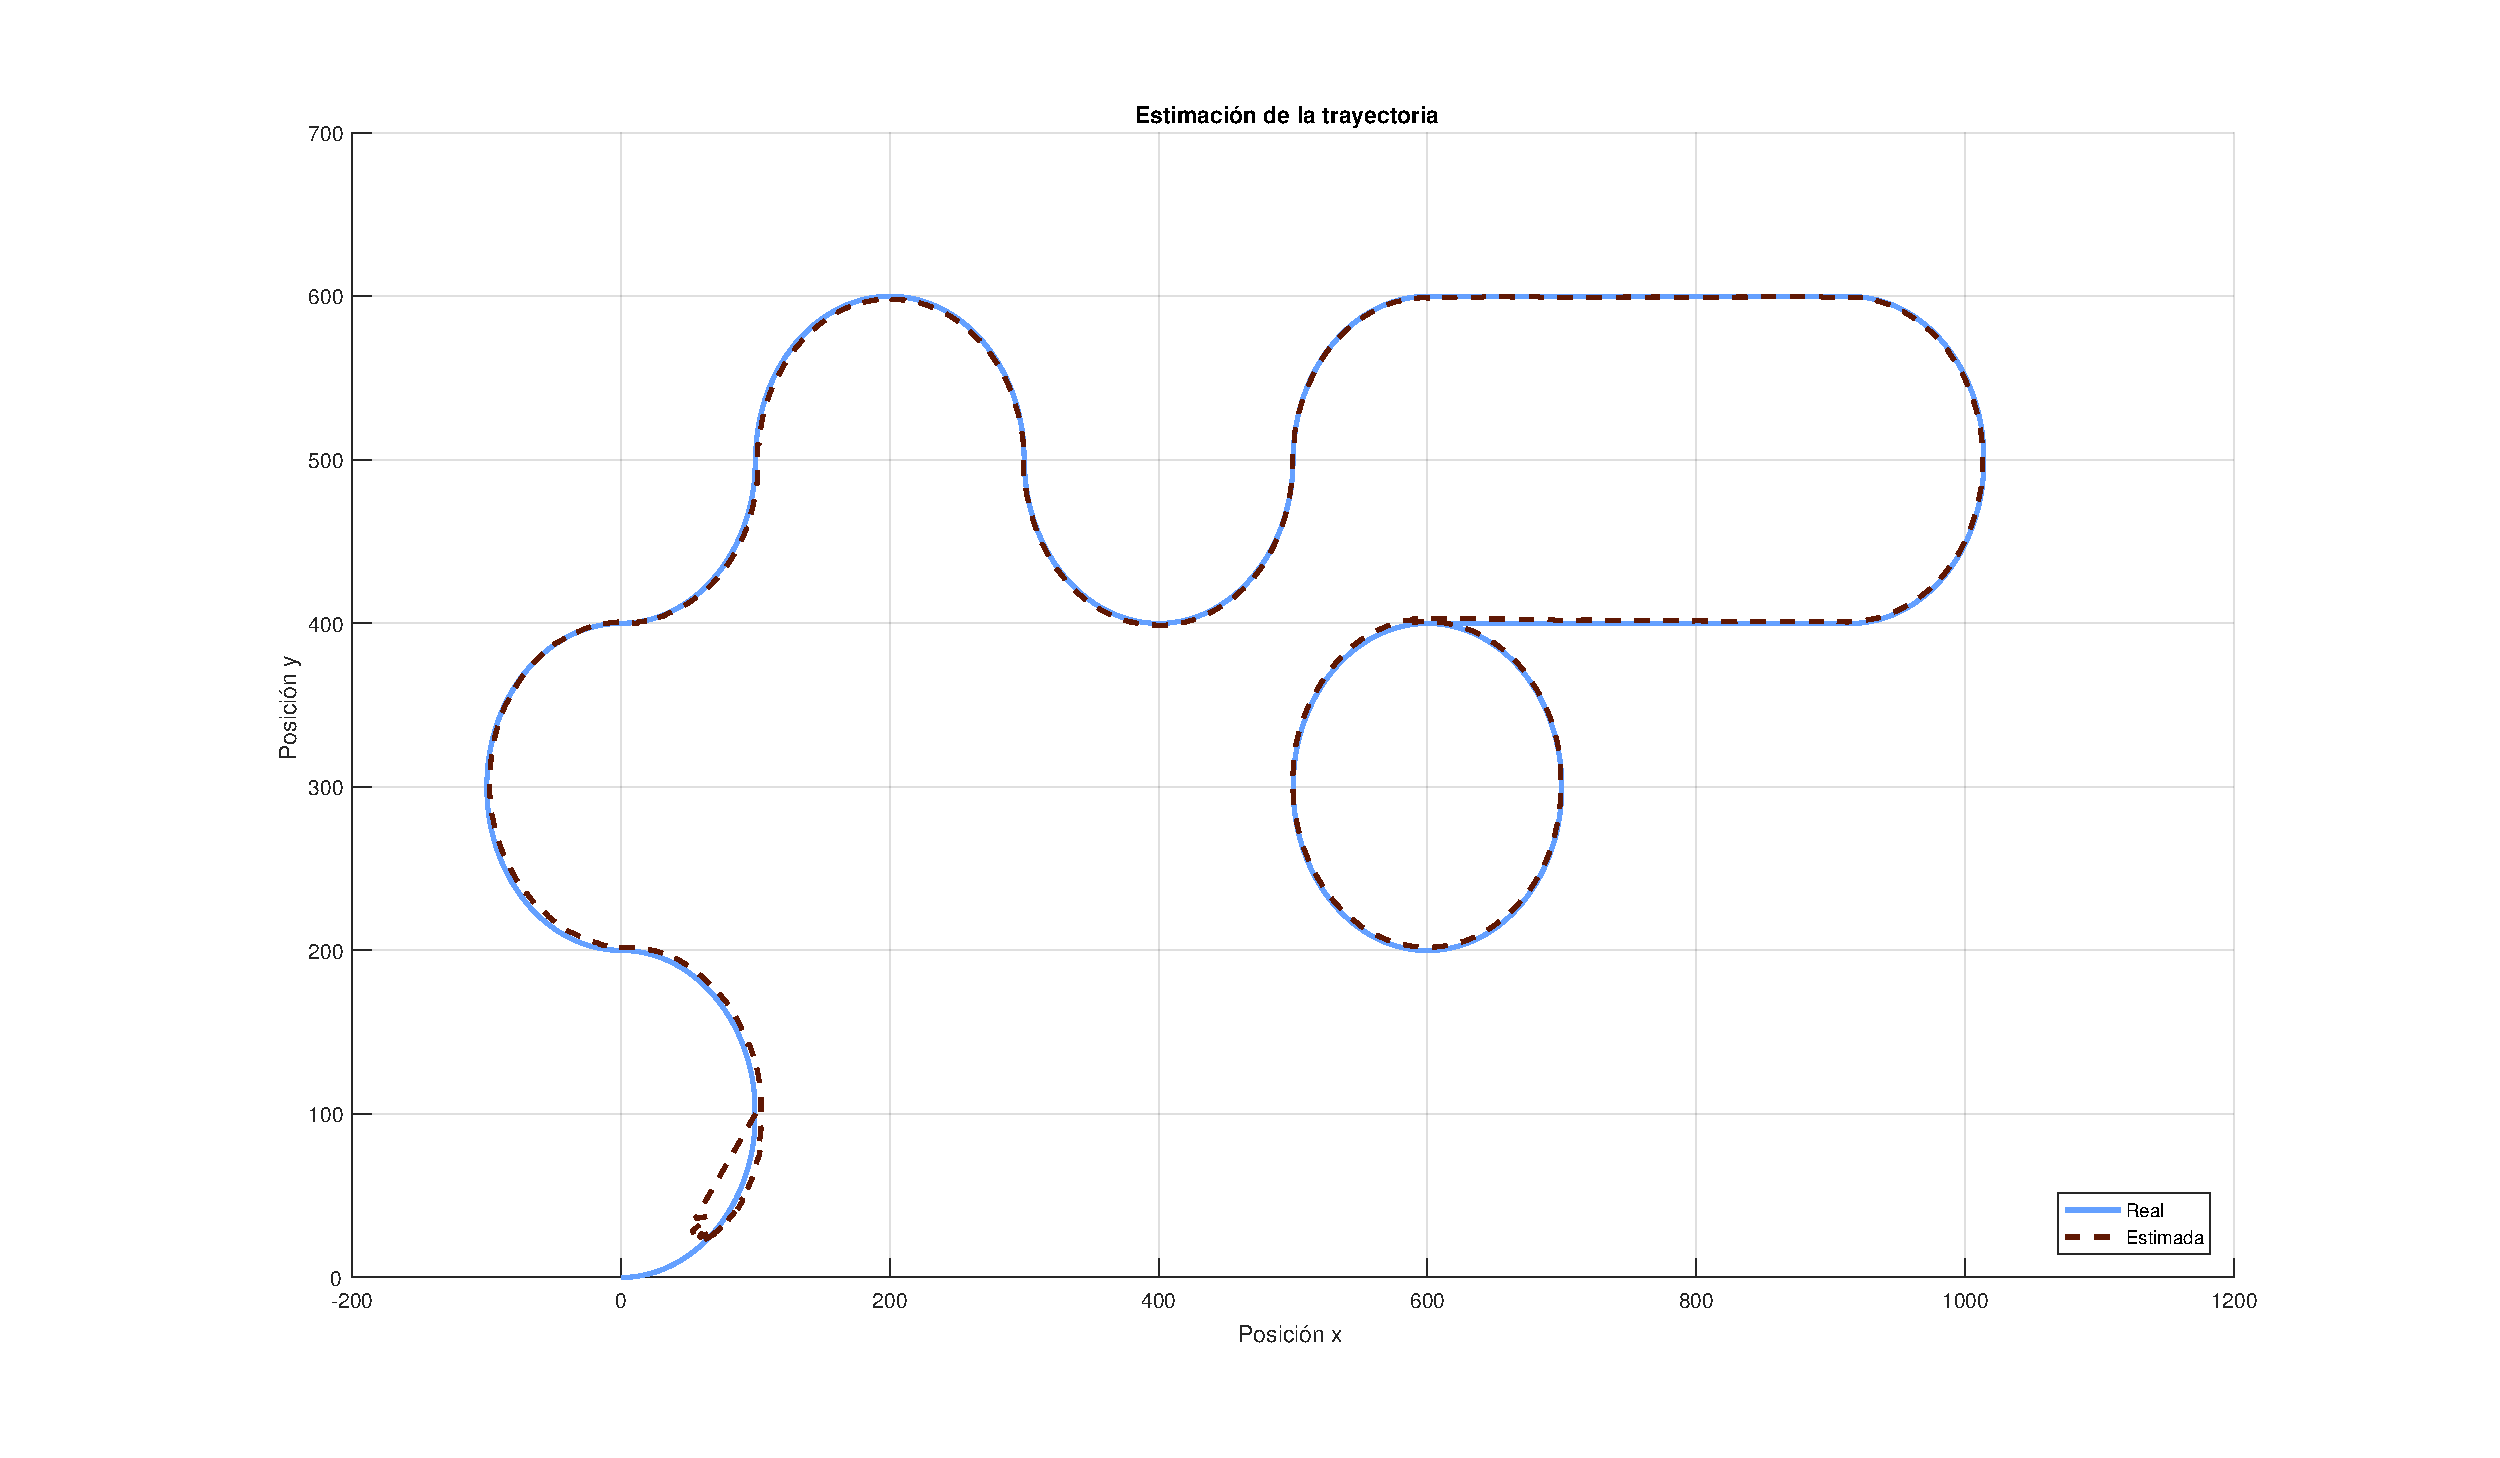
\includegraphics[width=\textwidth, trim= 2cm 2cm 2cm 2cm]{graf_ej2.pdf}
\caption{Estimación de la trayectoria.}
\label{fig:ej2} 
\end{figure}
	Al igual que en el trabajo práctico anterior, siendo todos los estados observables se obtiene una estimación muy buena de la trayectoria del vehículo como se expone en la Figura \ref{fig:ej2}. También se puede comprobar que el filtro de Kalman funciona correctamente al analizar las innovaciones (Figura \ref{fig:2covinn}). Se puede ver que la correlación de las mismas se asemeja al de un proceso blanco.
\graficarPDF{graf_ej2_covinn}{Innovaciones de las posiciones y velocidades en $x^e$ e $y^e$.}{fig:2covinn}
%\graficarPDFa{0 05cm 0 04cm}{graf_ej2_pos}{Posición y error de la misma en función del tiempo.}{fig:2pos}

\vspace*{\fill}
\begin{figure}[H]
\centering
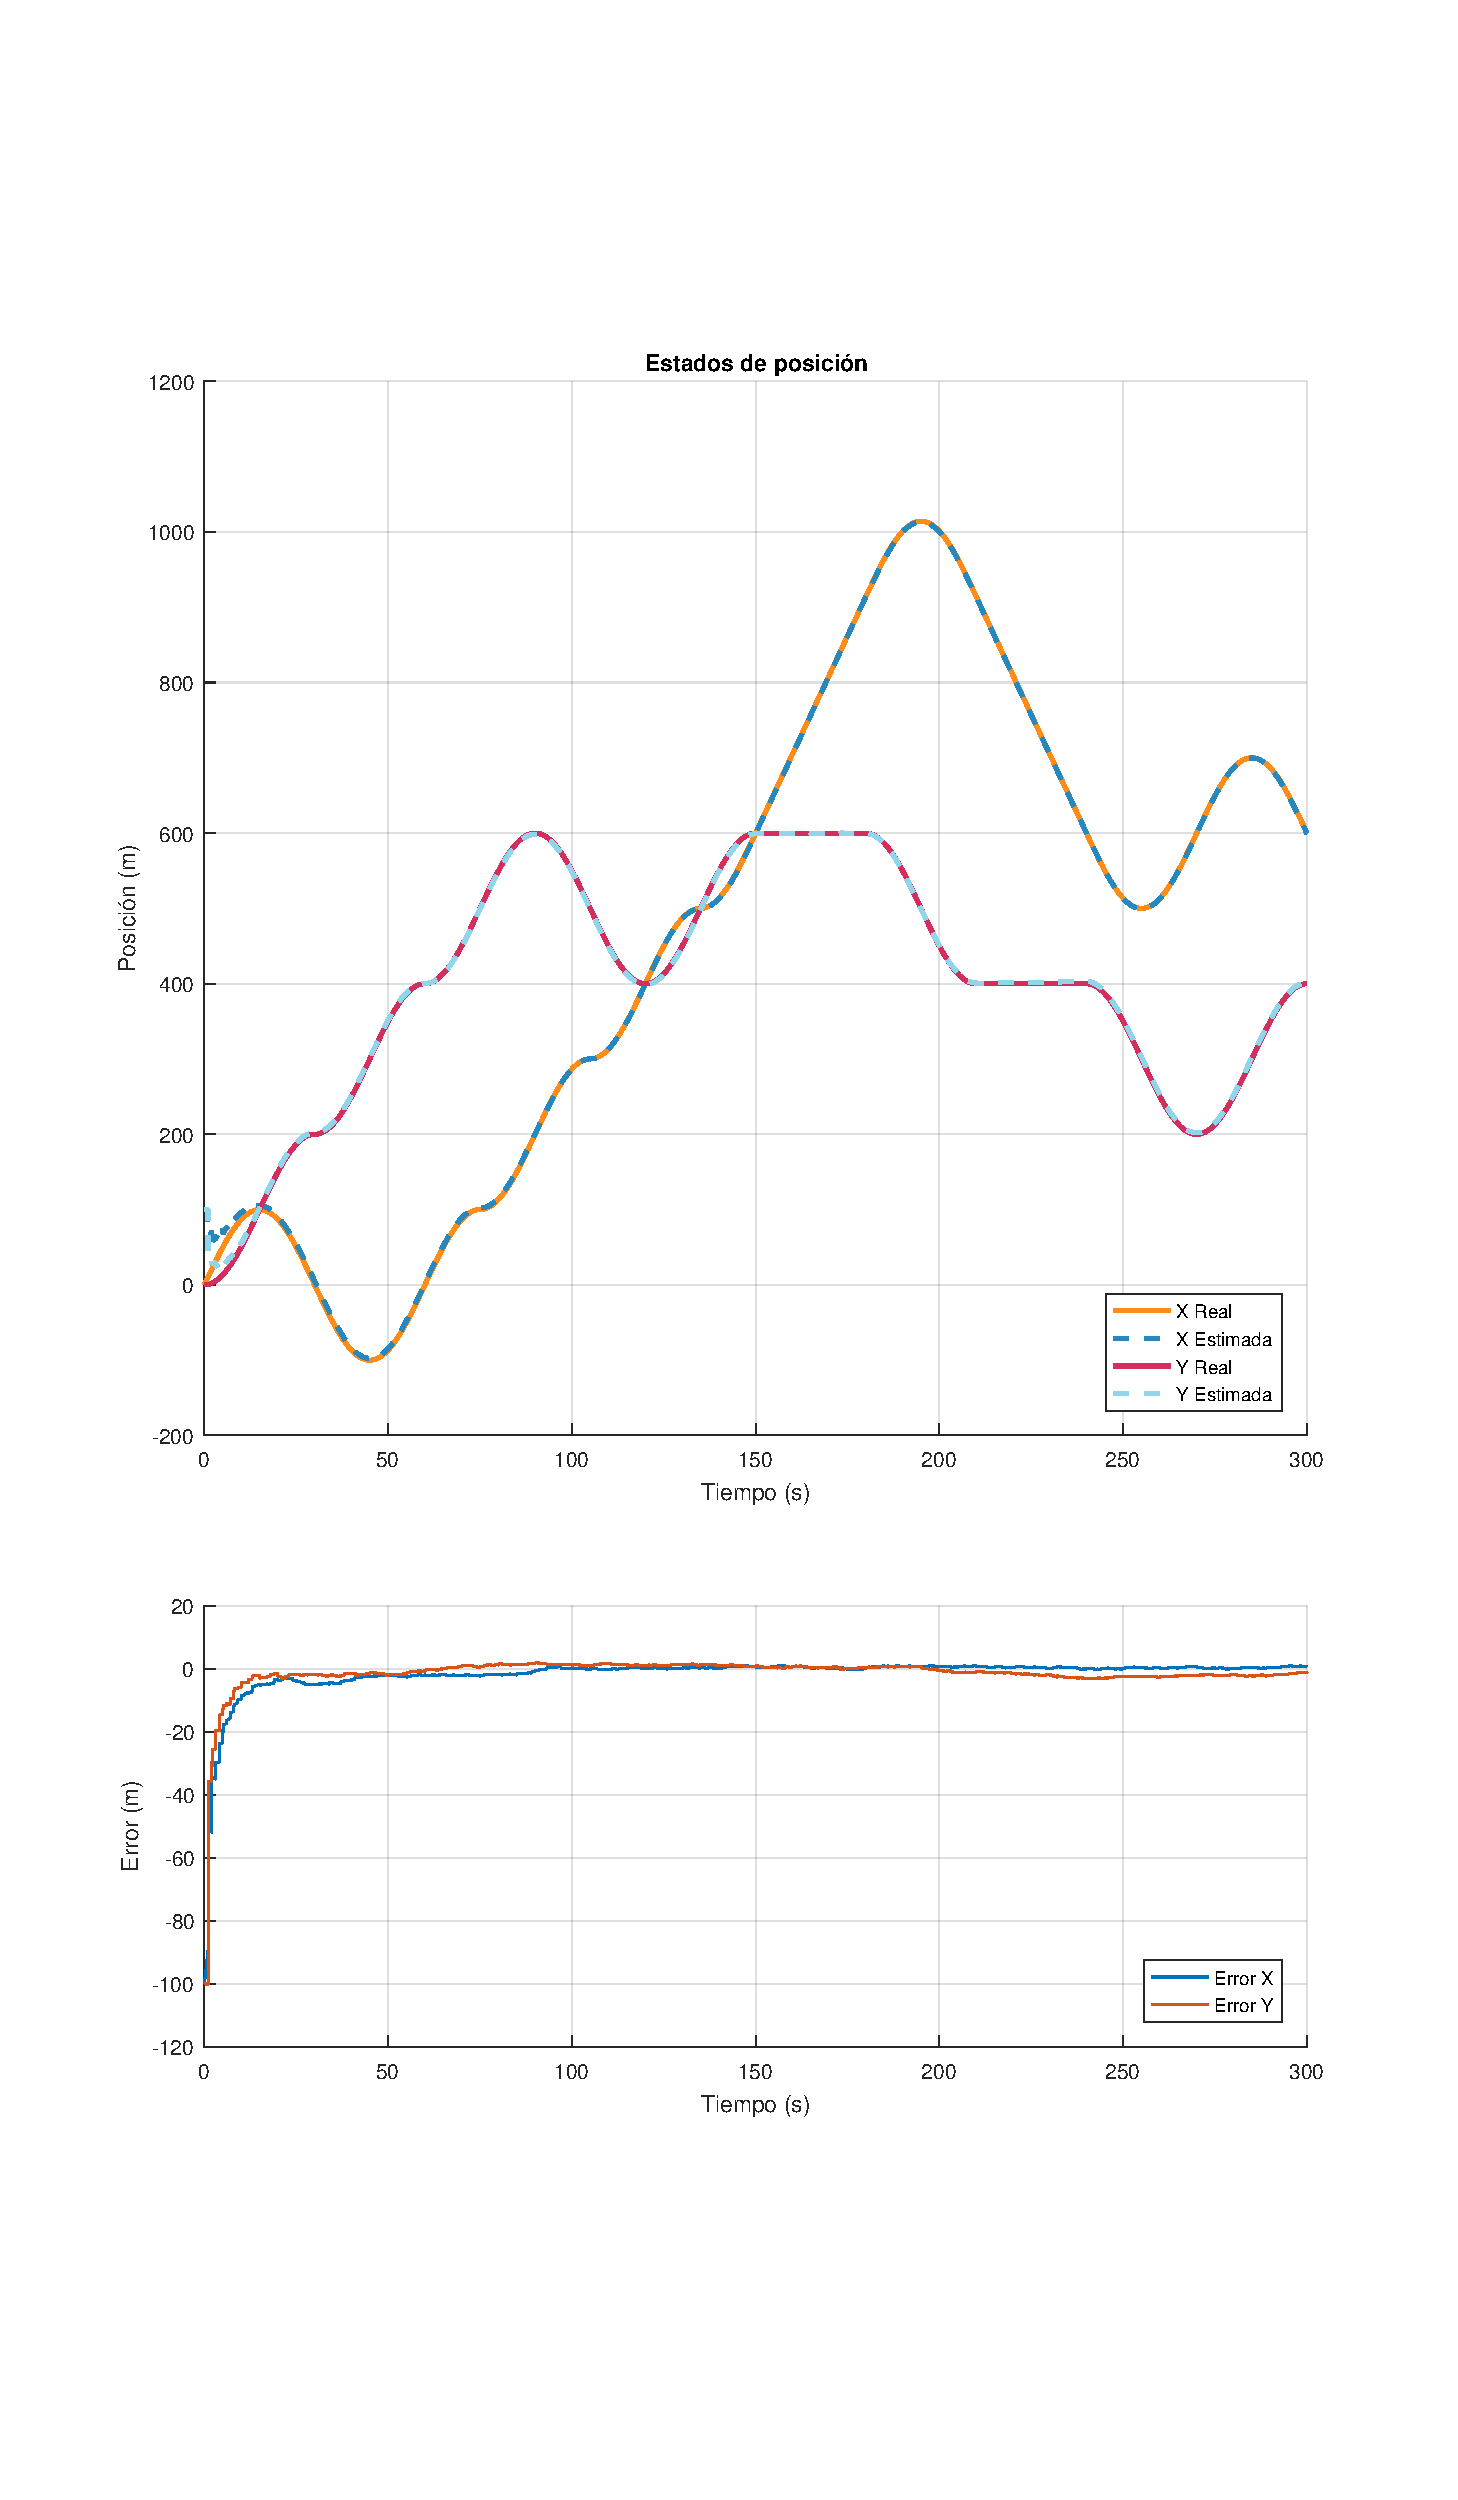
\includegraphics[scale=0.55, trim= 5cm 5cm 5cm 5cm]{graf_ej2_pos.pdf}
\caption{Posición y error de la misma en función del tiempo.}
\label{fig:2pos} 
\end{figure}
\vspace*{\fill}

	Analizando los gráficos de posición (Figura \ref{fig:2pos}) y velocidad (Figura \ref{fig:2vel}), en particular sus errores, se ve que tras un periodo pequeño de tiempo las estimaciones son iguales a los valores reales. En cuanto a las estimaciones de los coeficientes de la matriz de rotación expuestas en la Figura \ref{fig:2theta} se ve que el comportamiento es similar: comienzan con un error apreciable y converge rápidamente al valor real.

\vspace*{\fill}

\pagebreak

%\graficarPDF{graf_ej2_theta}{Valores de los coeficientes de $C^e_b$ en el tiempo.}{fig:2theta}

\vspace*{\fill}
\begin{figure}[H]
\centering
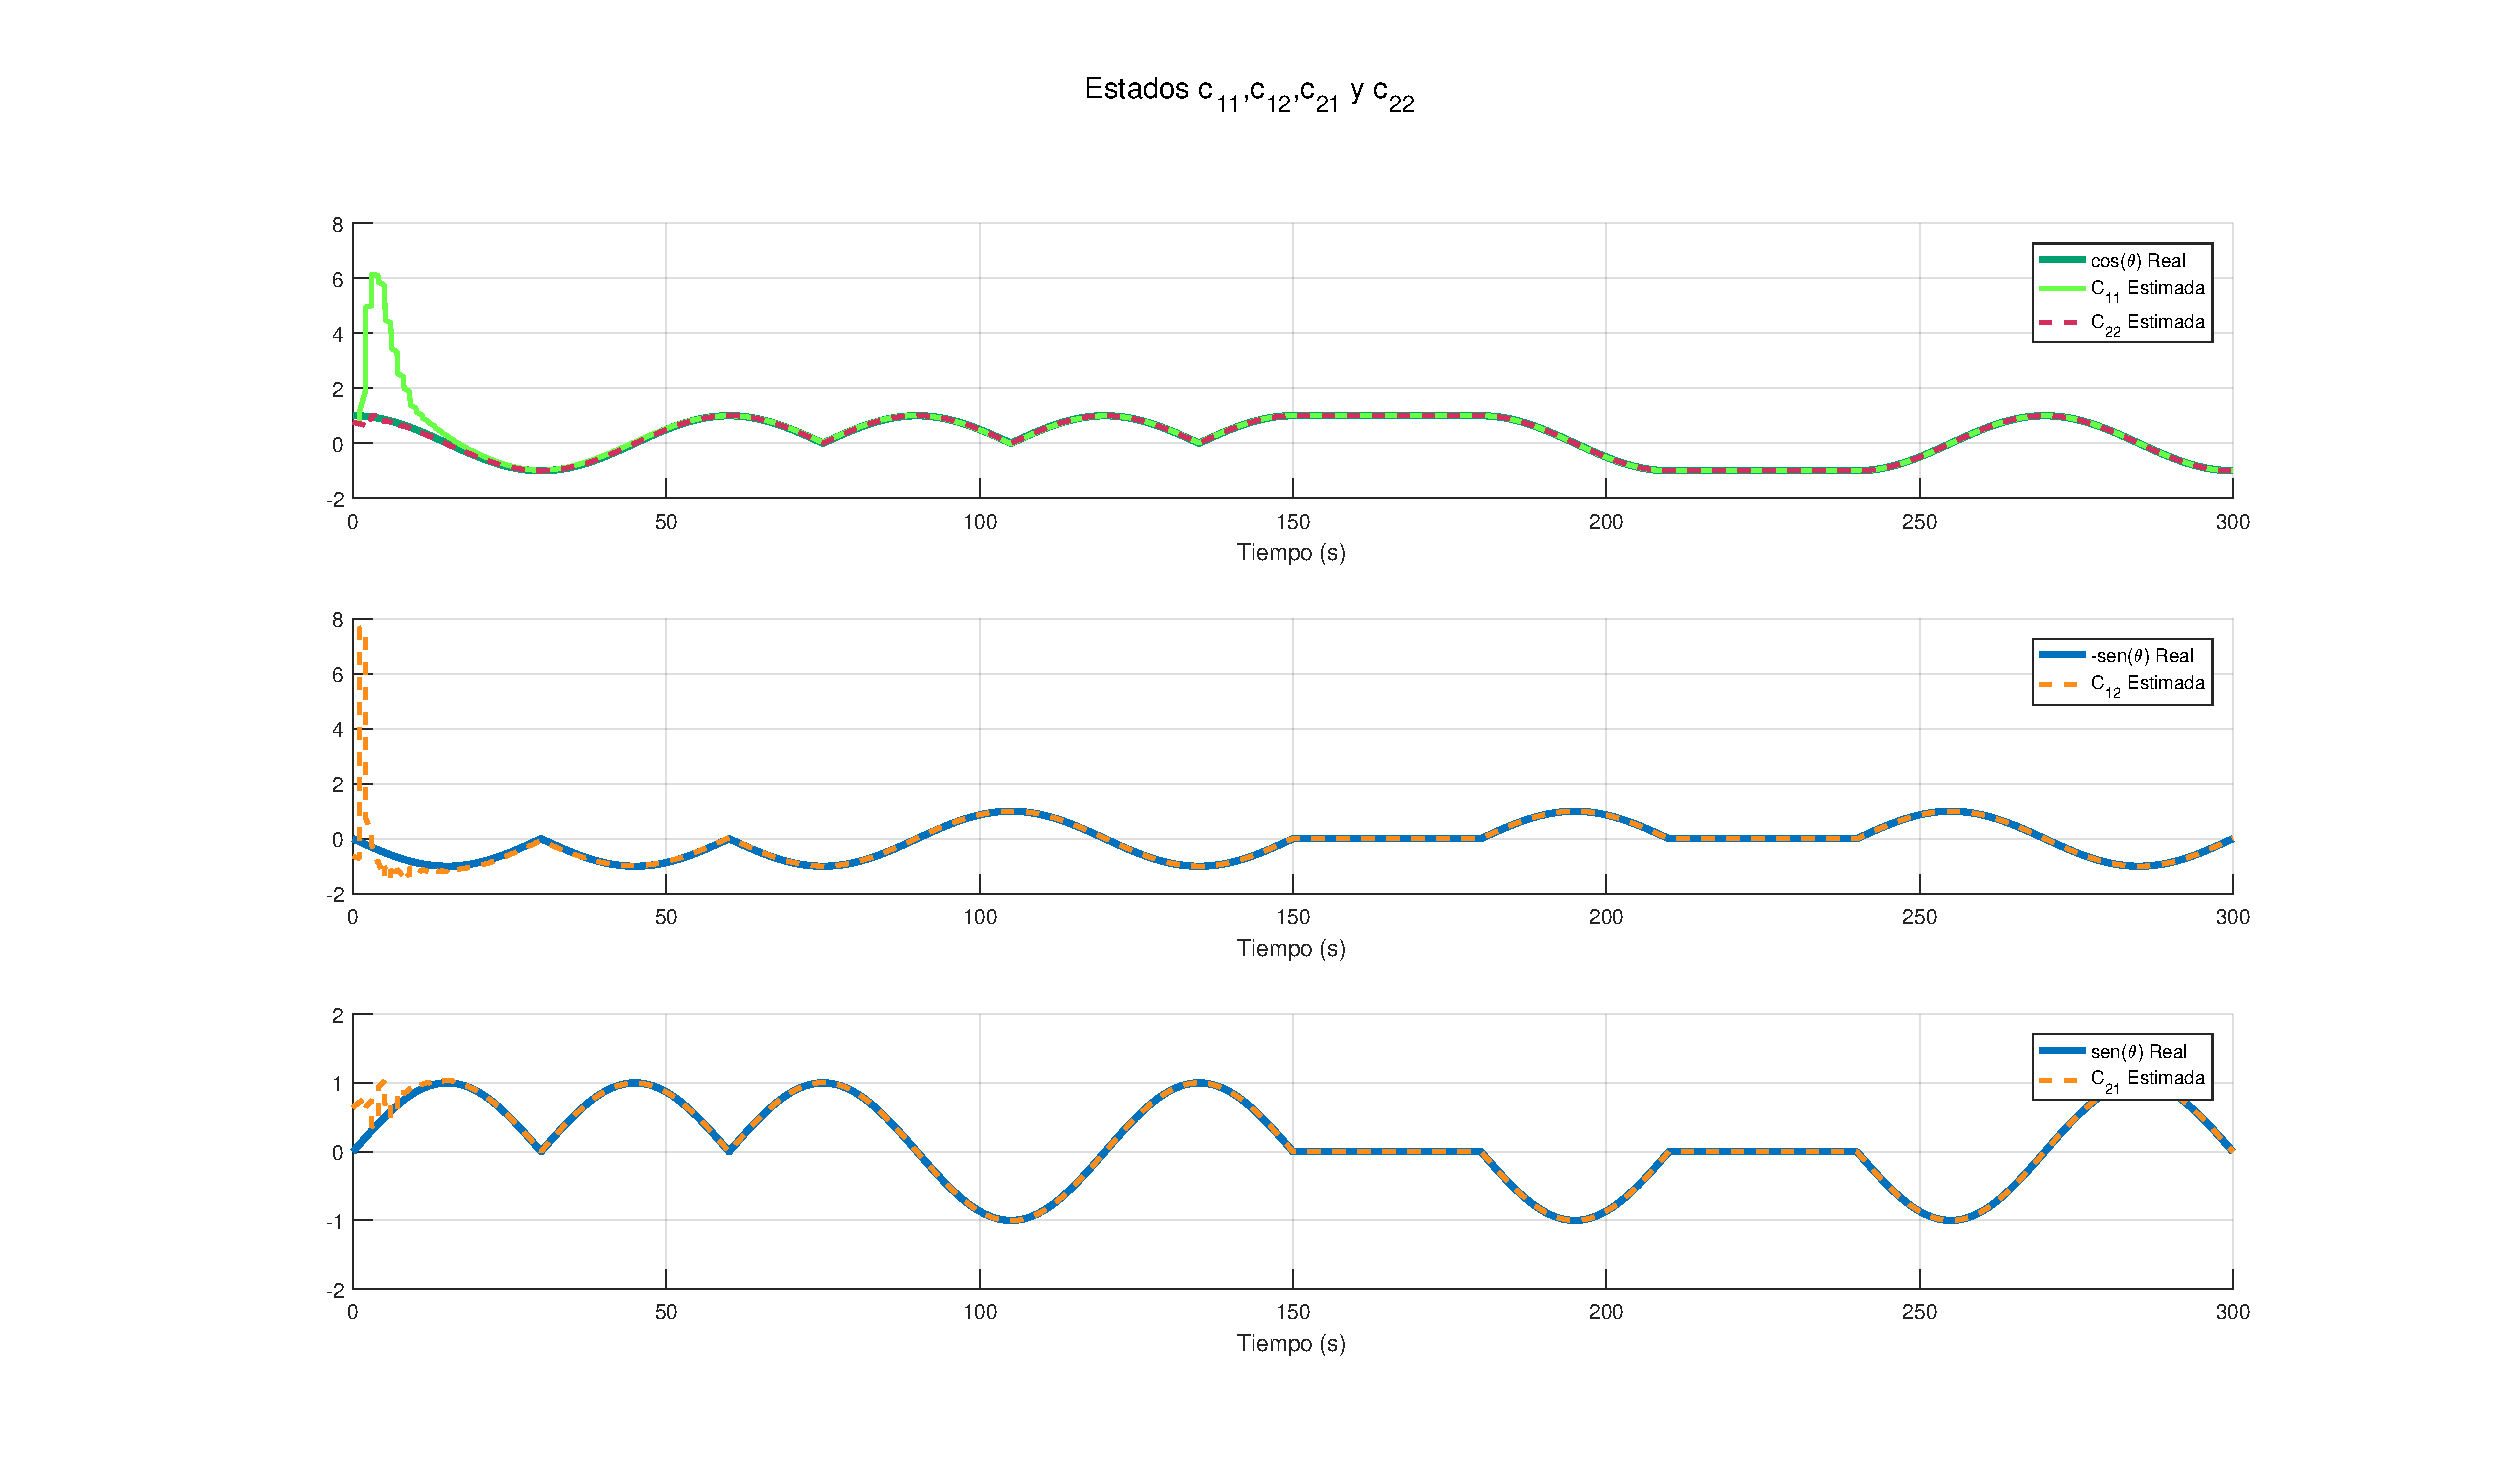
\includegraphics[width=\textwidth, trim= 2cm 2cm 2cm 2cm]{graf_ej2_theta.pdf}
\caption{Valores de los coeficientes de $C^e_b$ en el tiempo.}
\label{fig:2theta} 
\end{figure}
\vspace*{\fill}

%\graficarPDF{graf_ej2_vel}{Velocidad real y estimada en función del tiempo.}{fig:2vel}

\begin{figure}[H]
\centering
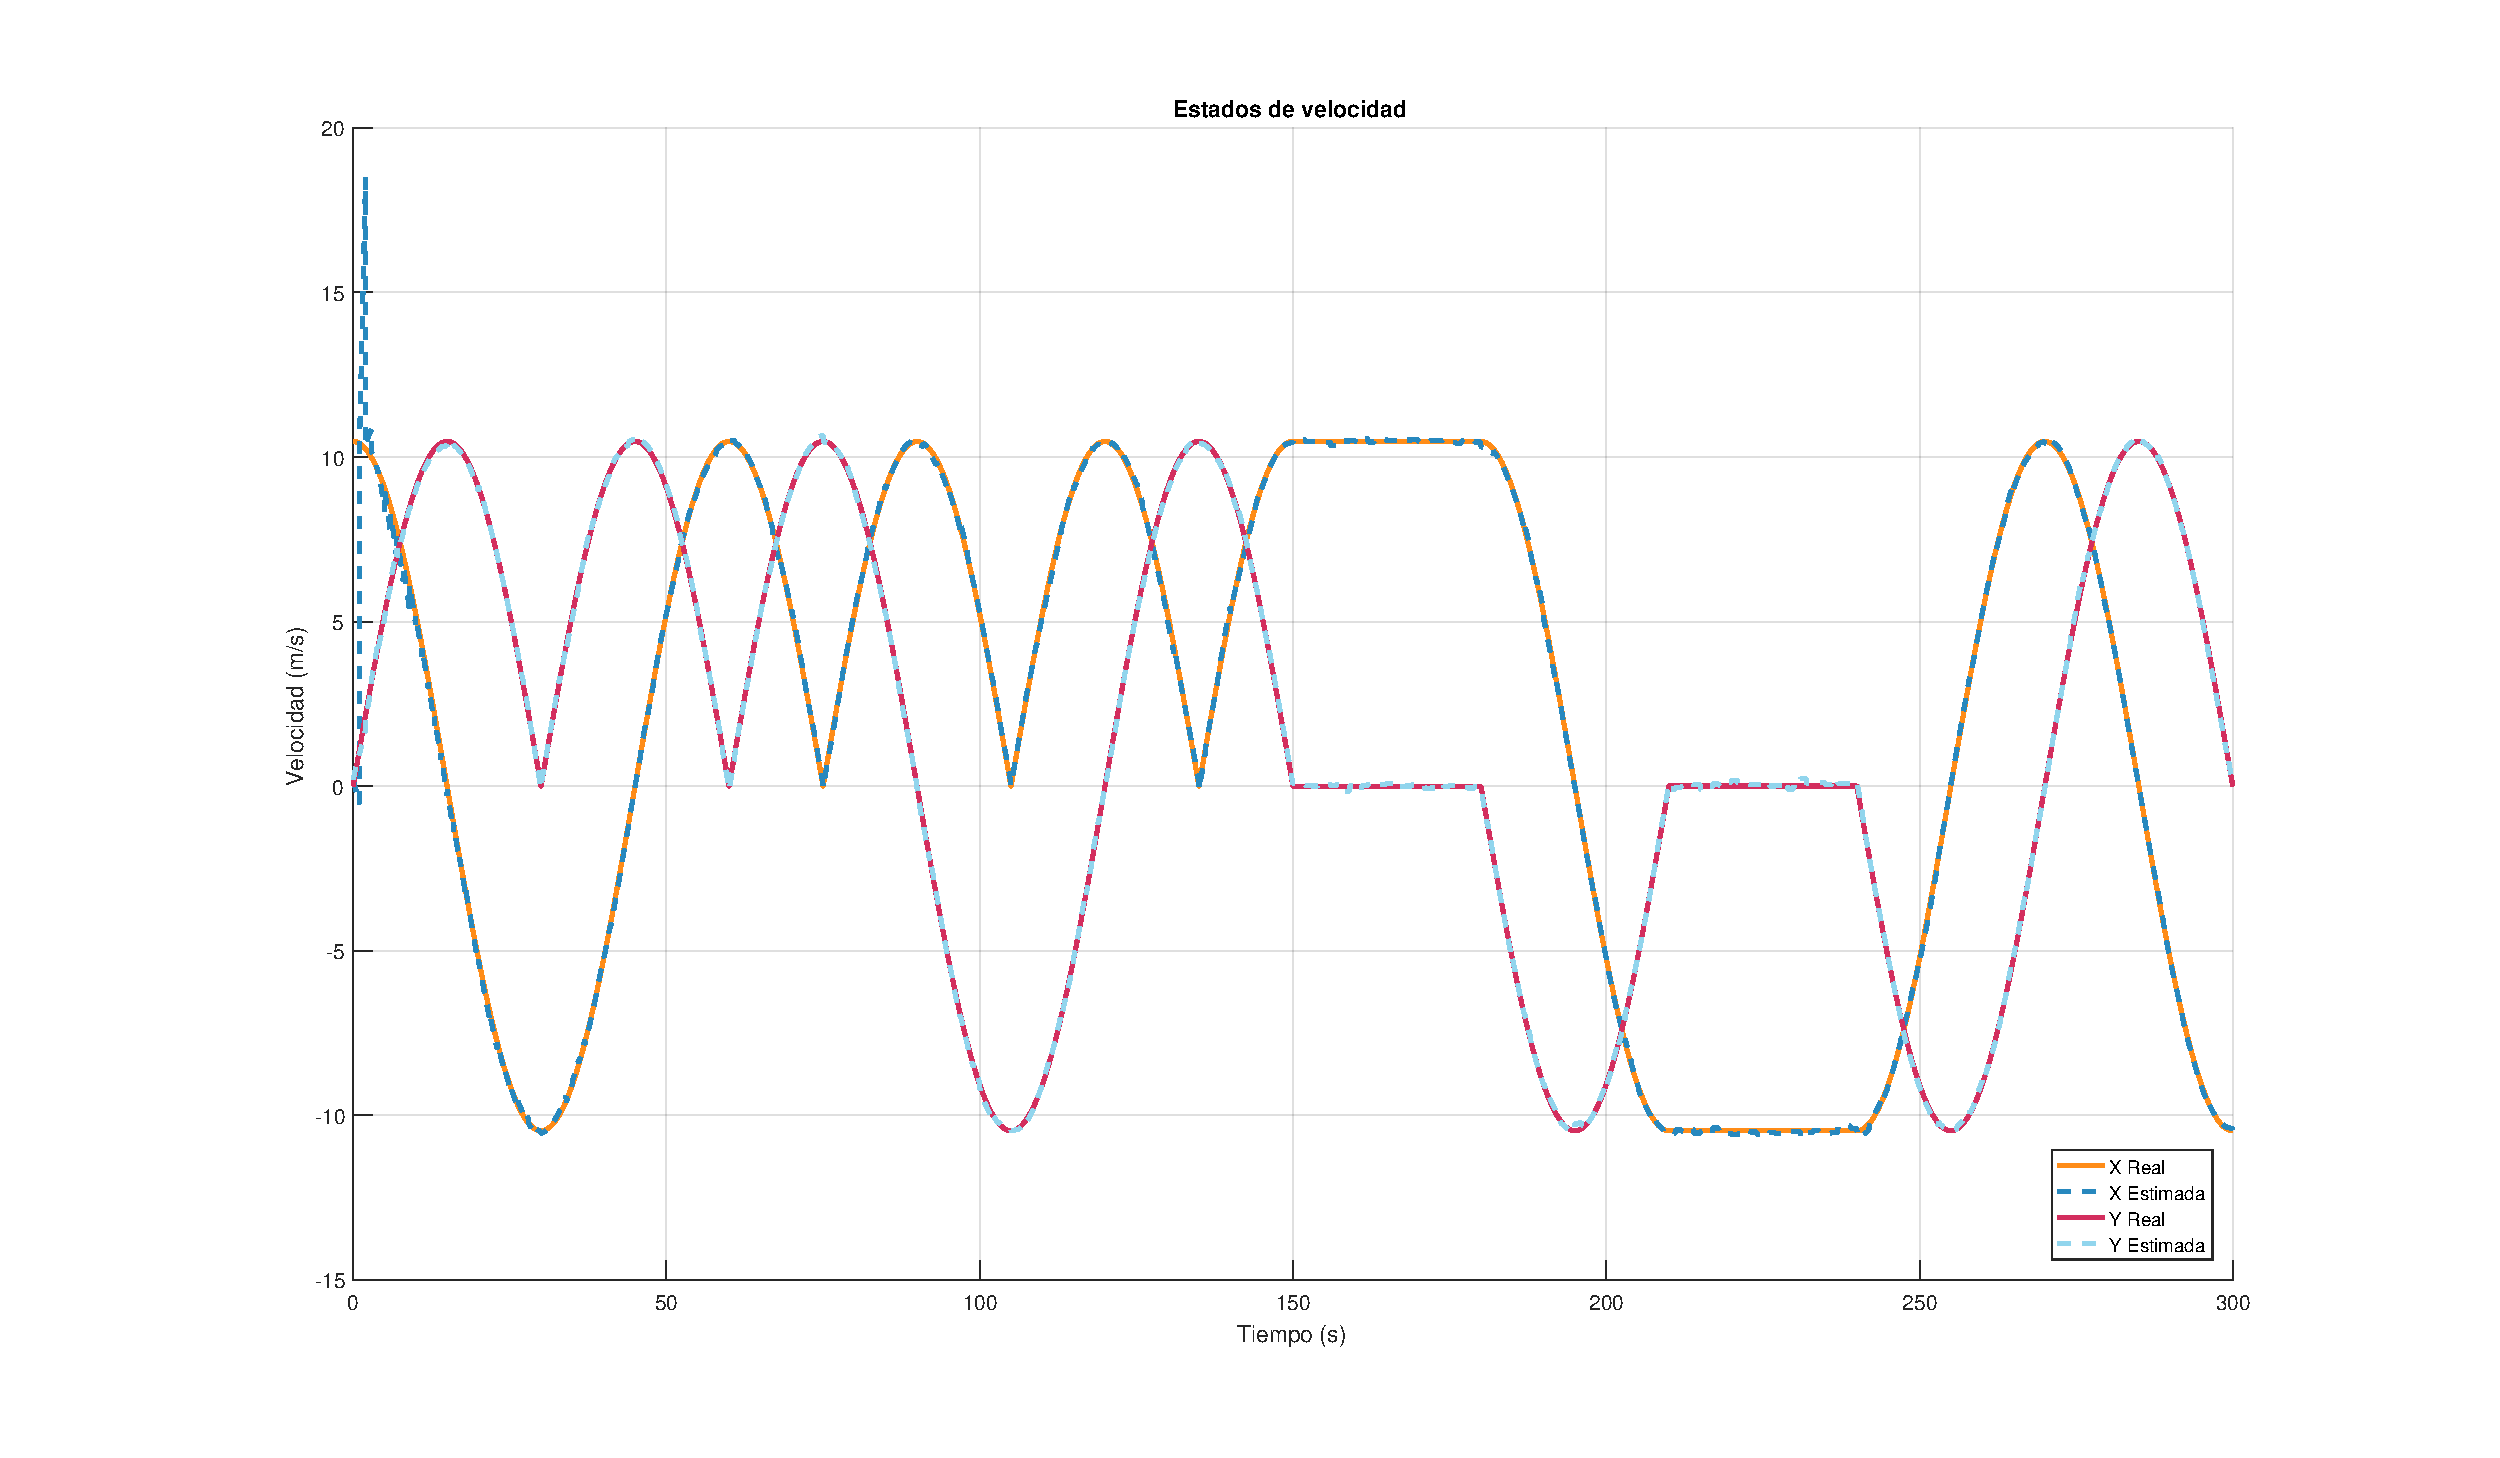
\includegraphics[width=\textwidth, trim= 2cm 2cm 2cm 2cm]{graf_ej2_vel.pdf}
\caption{Velocidad real y estimada en función del tiempo.}
\label{fig:2vel} 
\end{figure}
\vspace*{\fill}
